\documentclass[tikz,border=5pt]{standalone}
\usepackage{pgfplots}
\pgfplotsset{compat=1.18}

\definecolor{corba}{HTML}{365FB3}
\definecolor{secant}{HTML}{D97706}
\definecolor{tangent}{HTML}{15803D}

\begin{document}
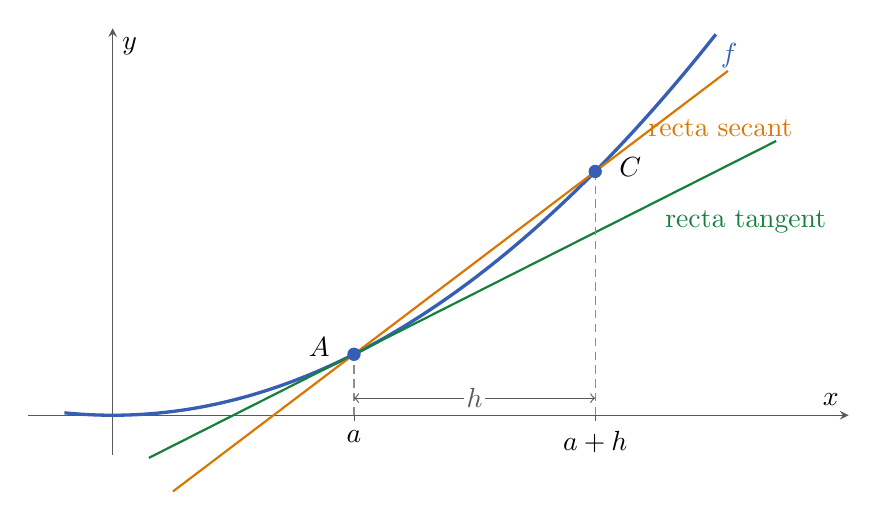
\begin{tikzpicture}
  \begin{axis}[
    width=12cm,
    height=7cm,
    axis lines=middle,
    xmin=-0.35,
    xmax=3.05,
    ymin=-0.65,
    ymax=6.35,
    xlabel={$x$},
    ylabel={$y$},
    xtick={1,2},
    xticklabels={$a$,$a+h$},
    ytick=\empty,
    axis line style={black!65},
    tick style={black!65},
    clip=false,
  ]
    % Funció de mostra: f(x)=x^2.
    \addplot[corba, very thick, domain=-0.2:2.5, samples=150] {x^2};
    \node[corba, anchor=west] at (axis cs:2.48,5.9) {$f$};

    % A=(a,f(a)), B=(a+h,f(a+h)), amb a=1 i h=1.
    \addplot[only marks, mark=*, mark size=2.2pt, corba]
      coordinates {(1,1) (2,4)};
    \node[anchor=east] at (axis cs:0.94,1.12) {$A$};
    \node[anchor=west] at (axis cs:2.06,4.08) {$C$};

    % Recta secant AB i recta tangent en A.
    \addplot[secant, thick, domain=0.25:2.55] {3*x-2};
    \node[secant, anchor=west] at (axis cs:2.18,4.72) {recta secant};
    \addplot[tangent, thick, domain=0.15:2.75] {2*x-1};
    \node[tangent, anchor=west] at (axis cs:2.25,3.18) {recta tangent};

    % Projeccions sobre l'eix horitzontal i increment h.
    \draw[densely dashed, black!45] (axis cs:1,0) -- (axis cs:1,1);
    \draw[densely dashed, black!45] (axis cs:2,0) -- (axis cs:2,4);
    \draw[<->, black!65]
      (axis cs:1,0.28) -- node[fill=white, inner sep=1pt] {$h$} (axis cs:2,0.28);
  \end{axis}
\end{tikzpicture}
\end{document}
